\chapter{Constraints satisfaction}

\begin{description}
    \item[Constraints satisfaction problem (CSP)] \marginnote{Constraints satisfaction problem (CSP)}
        Problem defined on a finite set of variables\\$(X_1, \dots, X_n)$,
        each belonging to a domain $(D_1, \dots, D_n)$ 
        (notation: $X_i :: [d_{i,1}, \dots, d_{i,m}]$ or $X_i \in [d_{i,1}, \dots, d_{i,m}]$).

        A constraint is a relationship between variables (e.g. $X < Y$). 
        Formally, a constraint $c(X_{k_1}, \dots, X_{k_m})$ is a subset of the cartesian product
        $D_{k_1} \times \dots \times D_{k_m}$ of the admissible values of the variables.

        A solution to a CSP is an admissible assignment of all the variables.

        CSP can be solved as a search problem.
        \begin{descriptionlist}
            \item[A posteriori algorithms] \marginnote{A posteriori algorithms}
                Constraints are checked after the construction of the search tree.
        
            \item[Propagation algorithms] \marginnote{Propagation algorithms}
                Once a variable has been assigned, 
                constraints are propagated to the unassigned variables to prune part of the search space.
        
            \item[Consistency techniques] \marginnote{Consistency techniques}
                Constraints are propagated to derive a simpler problem.
        \end{descriptionlist}
\end{description}



\section{A posteriori algorithms}

\subsection{Generate and test}
\marginnote{Generate and test}

The search tree is constructed depth-first. 
At level $i$, a value is assigned to the variable $X_i$.
Constraints are only checked when a leaf has been reached.

In other words, it computes all the permutations of the values of the variables.


\subsection{Standard backtracking}
\marginnote{Standard backtracking}

The search tree is constructed depth-first. 
At level $i$, a value is assigned to the variable $X_i$ and 
constraints involving $X_1, \dots, X_i$ are checked.
In case of failure, the path is not further explored.

A problem with this approach is that it requires to backtrack in case of failure
and reassign all the variables in the worst case.



\section{Propagation algorithms}

\subsection{Forward checking}
\marginnote{Forward checking}

The search tree is constructed depth-first. 
At level $i$, a value is assigned to the variable $X_i$ and 
constraints involving $X_i$ are propagated
to restrict the domain of the remaining unassigned variables.
If the domain of a variable becomes empty, the path is considered a failure and the algorithm backtracks.

\begin{example}
    Consider the variables: 
    \[ X_1 :: [1, 2, 3] \hspace{1cm} X_2 :: [1, 2, 3] \hspace{1cm} X_3 :: [1, 2, 3] \]
    and the constraints $X_1 < X_2 < X_3$.

    We assign the variables in lexicographic order, at each step we have that:
    \begin{enumerate}
        \item $X_1 = 1 \hspace{1cm} X_2 :: [\cancel{1}, 2, 3] \hspace{1cm} X_3 :: [\cancel{1}, 2, 3]$
        \item $X_1 = 1 \hspace{1cm} X_2 = 2 \hspace{1cm} X_3 :: [\cancel{1}, \cancel{2}, 3]$
        \item $X_1 = 1 \hspace{1cm} X_2 = 2 \hspace{1cm} X_3 = 3$
    \end{enumerate}

    In another scenario, assume that we choose $X_1 = 2$ as first step:
    \begin{enumerate}
        \item $X_1 = 2 \hspace{1cm} X_2 :: [\cancel{1}, \cancel{2}, 3] \hspace{1cm} X_3 :: [\cancel{1}, \cancel{2}, 3]$
        \item $X_1 = 2 \hspace{1cm} X_2 = 3 \hspace{1cm} X_3 :: [\cancel{1}, \cancel{2}, \cancel{3}]$
    \end{enumerate}
    As the domain of $X_3$ is empty, a search on this branch fails and backtracking is required.
\end{example}



\subsection{Look ahead}

\begin{description}
    \item[Partial look ahead (PLA)] \marginnote{Partial look ahead (PLA)}
        When a variable $X_i$ has been assigned, it is propagated to unassigned variables (as in forward checking).
        Then, for each unassigned variable $X_h$, we check its values against the ones of the variables $X_{h+1}, \dots, X_{n}$ in front of it 
        (note that the check is not done in both directions).
        
        When checking the values of an unassigned variable $X_p :: D_p$ against $X_q :: D_q$, 
        we maintain a value $x \in D_p$ only if there is at least a corresponding value $y \in D_q$ such that 
        an assignment $X_p=x$ and $X_q=y$ does not violate the constraints. 
        $y$ is called support \marginnote{Support} of $x$. 

        \begin{example}
            Consider the variables and constraints: 
            \[ X_1 :: [1, 2, 3] \hspace{0.5cm} X_2 :: [1, 2, 3] \hspace{0.5cm} X_3 :: [1, 2, 3]  \hspace{1cm}  X_1 < X_2 < X_3 \]

            We assign the variables in lexicographic order. At each step, we have that:
            \begin{enumerate}
                \item $X_1 = 1 \hspace{1cm} X_2 :: [\cancel{1}, 2, \cancel{3}] \hspace{1cm} X_3 :: [\cancel{1}, 2, 3]$ \\
                    Here, we assign $X_1=1$ and propagate to unassigned constraints.
                    Then, we check the constraints of $(X_2, X_3)$: $X_2 = 3$ is not possible as it does not have a support in $X_3$.
                \item $X_1 = 1 \hspace{1cm} X_2 = 2 \hspace{1cm} X_3 :: [\cancel{1}, \cancel{2}, 3]$
                \item $X_1 = 1 \hspace{1cm} X_2 = 2 \hspace{1cm} X_3 = 3$
            \end{enumerate}
        \end{example}

    \item[Full look ahead (FLA)] \marginnote{Full look ahead (FLA)}
        Same as partial look ahead, but the checks on unassigned variables are bidirectional.

        \begin{example}
            Consider the variables and constraints: 
            \[ X_1 :: [1, 2, 3] \hspace{0.5cm} X_2 :: [1, 2, 3] \hspace{0.5cm} X_3 :: [1, 2, 3]  \hspace{1cm}  X_1 < X_2 < X_3 \]

            We assign the variables in lexicographic order. At each step, we have that:
            \begin{enumerate}
                \item $X_1 = 1 \hspace{1cm} X_2 :: [\cancel{1}, 2, \cancel{3}] \hspace{1cm} X_3 :: [\cancel{1}, \cancel{2}, 3]$ \\
                    Here, we assign $X_1=1$ and propagate to unassigned constraints.
                    Then, we check the constraints of:
                    \begin{itemize}
                        \item $(X_2, X_3)$: $X_2 = 3$ is not possible as it does not have a support in $X_3$.
                        \item $(X_3, X_2)$: $X_3 = 2$ is not possible as it does not have a support in $X_2$.
                    \end{itemize} 
                    Note that checking in a different order might result in different (but correct) domains.
                \item $X_1 = 1 \hspace{1cm} X_2 = 2 \hspace{1cm} X_3 = 3$
            \end{enumerate}
        \end{example}
\end{description}



\section{Search heuristics}
When searching, we have two degrees of freedom:
\begin{enumerate}
    \item Selection of the variable to assign.
    \item Selection of the value to assign.
    \item Strategy for propagation.
\end{enumerate}

Heuristics can be used to make better selections (for the points 1. and 2.):
\begin{descriptionlist}
    \item[Variable selection] \marginnote{Variable selection heuristics}
        \phantom{}
        \begin{description}
            \item[First-fail (minimum remaining values)] \marginnote{First-fail}
                Choose the variable with the smallest domain.

            \item[Most-constrained principle] \marginnote{Most-constrained principle}
                Choose the variable that appears the most in the constraints. 
                In this way, harder variables are ideally assigned first.
        \end{description}

    \item[Value selection] \marginnote{Value selection heuristics}
        The choice of the value to assign to a variable does not have general rules.
\end{descriptionlist}

Moreover, heuristics can be:
\begin{descriptionlist}
    \item[Static] \marginnote{Static heuristics} 
        Computed before the search. 
    
    \item[Dynamic] \marginnote{Dynamic heuristics} 
        Can be computed at each assignment.
\end{descriptionlist}



\section{Consistency techniques}

Consistency techniques reduce the original problem by removing domain values that are surely impossible.
This class of methods can be applied statically before the search or after each assignment.

\begin{description}
    \item[Constraint graph] \marginnote{Constraint graph}
        Graph where nodes are variables and arcs are constraints.
        \begin{itemize}
            \item There is a directed arc from $X_i$ to $X_j$ if there is a binary constraint $X_i \circ X_j$.
            \item There is a self-loop to $X_i$ if there is a unary constraint on $X_i$.
        \end{itemize}

    \item[Node consistency (level 1 consistency)] \marginnote{Node consistency}
        A node $X_i$ is consistent if all of its values in the domain satisfy the constraints.

        A graph is node consistent if all its nodes are consistent.

    \item[Arc consistency (level 2 consistency)] \marginnote{Arc consistency}
        An arc from $X_i :: D_i$ to $X_j :: D_j$ is consistent if each value of $D_i$ has a support in $D_j$ (as in look ahead).

        A graph is arc consistent if all its arcs are consistent.

        \begin{description}
            \item[AC-3 algorithm] \marginnote{AC-3 algorithm}
                A possible algorithm to achieve arc consistency.
                Uses a queue to store arcs to explore:
                \begin{enumerate}
                    \item At the beginning, all arcs are in the queue. 
                    \item When evaluating an arc $(X_i, X_j)$, 
                        values in the domain of $X_i$ are removed if they don't have a support in the domain of $X_j$.
                    \item If the domain of $X_i$ has been modified, 
                        for all the neighbors $X_k$ of $X_i$, the arc $(X_k, X_i)$ is added to the queue.
                    \item Repeat until empty queue (quiescence).
                \end{enumerate} 
            \end{description}

        \begin{example}
            Note: when doing the exercises, it is sufficient to iterate until none of the nodes change, without using a queue.
            
            Consider the variables and constraints: 
            \[ X_1 :: [1, 2, 3] \hspace{0.5cm} X_2 :: [1, 2, 3] \hspace{0.5cm} X_3 :: [1, 2, 3]  \hspace{1cm}  X_1 < X_2 < X_3 \]
            The constraint graph and the iterations to achieve arc consistency are the following:

            \begin{minipage}{0.7\textwidth}
                \begin{enumerate}
                    \item We check the following pairs:
                        \begin{itemize}
                            \item $(X_1, X_2)$. Here, $X_1 :: [1, 2, \cancel{3}]$.
                            \item $(X_2, X_1)$. Here, $X_2 :: [\cancel{1}, 2, 3]$.
                            \item $(X_2, X_3)$. Here, $X_2 :: [\cancel{1}, 2, \cancel{3}]$.
                            \item $(X_3, X_2)$. Here, $X_3 :: [\cancel{1}, \cancel{2}, 3]$.
                            \item $(X_1, X_3)$. Here, $X_1 :: [1, 2, \cancel{3}]$ (no changes).
                            \item $(X_3, X_1)$. Here, $X_3 :: [\cancel{1}, \cancel{2}, 3]$ (no changes).
                        \end{itemize}
                        The resulting domains are:
                        \[ X_1 :: [1, 2, \cancel{3}] \hspace{0.5cm} X_2 :: [\cancel{1}, 2, \cancel{3}] \hspace{0.5cm} X_3 :: [\cancel{1}, \cancel{2}, 3] \]
                    \item We check the following pairs:
                        \begin{itemize}
                            \item $(X_1, X_2)$. Here, $X_1 :: [1, \cancel{2}, \cancel{3}]$.
                            \item Other pairs do nothing.
                        \end{itemize}
                        The resulting domains are:
                        \[ X_1 :: [1, \cancel{2}, \cancel{3}] \hspace{0.5cm} X_2 :: [\cancel{1}, 2, \cancel{3}] \hspace{0.5cm} X_3 :: [\cancel{1}, \cancel{2}, 3] \]
                \end{enumerate}
            \end{minipage}
            \begin{minipage}{0.20\textwidth}
                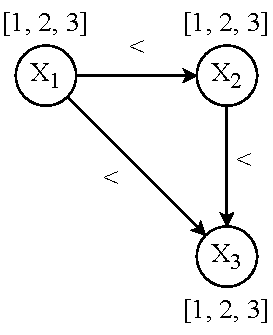
\includegraphics[width=\linewidth]{img/_constraint_graph.pdf}
            \end{minipage}
        \end{example}

    \item[Path consistency (level 3 consistency)] \marginnote{Path consistency}
        A path $(X_i, X_j, X_k)$ is path consistent if $X_i$ and $X_j$ are node consistent, $(X_i, X_j)$ is arc consistent and
        for every pair of values in the domains of $X_i$ and $X_j$, there is a support in the domain of $X_k$.

    \item[K-consistency] \marginnote{K-consistency}
        Generalization of arc/path consistency.
        If a problem with $n$ variables is $n$-consistent, the solution can be found without search.

        Usually, it is not applicable as it has exponential complexity.
\end{description}